\documentclass[a4paper,11pt]{report}
\usepackage{hyperref}
\usepackage{appendix}
\usepackage{listings}
\usepackage{fancybox}
\usepackage{graphicx}
\graphicspath{ {images/} }
\usepackage{parskip}
\usepackage{index}
\makeindex
\makeatletter
\newcommand{\head}[1]{\textbf{#1}}
\newenvironment{CenteredBox}{% 
\begin{Sbox}}{% Save the content in a box
\end{Sbox}\centerline{\parbox{\wd\@Sbox}{\TheSbox}}}% And output it centered
\makeatother
\lstset{
	basicstyle=\ttfamily\scriptsize,
	breaklines=true,
	showstringspaces=false
}
\renewcommand{\bibname}{References}
\begin{document}
\begin{titlepage}
	\centering
	{\bfseries Component Based MMIX Simulator using Multiple Programming Paradigms \par}
	\vspace{1cm}
	{A dissertation submitted in partial fulfillment of the requirements for the MSc in Advanced Computing Technologies\par}
	\vspace{1.5cm}
	{by Stephen Edmans\par}
	\vspace{2cm}
	{Department of Computer Science and Information Systems\par}
	{Birkbeck College, University of London\par}
	\vspace{2cm}
	{\large September 2015\par}
\end{titlepage}
\newpage
\chapter*{} % Academic Declaration
{This report is substantially the result of my own work except where explicitly
indicated in the text. I give my permission for it to be submitted to the JISC
Plagiarism Detection Service. I have read and understood the sections on plagiarism
in the Programme Handbook and the College website.\par}
\vspace{1cm}
{\noindent The report may be freely copied and distributed provided the source is explicitly
acknowledged.}
\chapter*{Abstract}
\addcontentsline{toc}{chapter}{Abstract}

There are currently over 2,500\footnote{From the language list\cite{numlangs}} different programming languages, with more created every year. These programming languages can get grouped together in numerous different ways.  This makes the decision of what language to use when starting a new project extremely difficult.

There are several ways in which we can reach this decision; choose the language that your team knows best; choose the language that makes the most sense to implement the critical part of your system; choose a simple general purpose language; choose a language that has got an active community. There is no acknowledged best approach to take.

Another approach would be to split your application up into separate components and using a different programming language for each component. This allows us choose the most appropriate programming language for each component.

The purpose of this project is to examine this approach. The application that we will create will be a simulator for an artificial machine language. The artificial machine language that we will use is called MMIX, it was developed by Donald Knuth as part of his seminal work The Art of Computer Programming\cite{knuth:aocp1}.
\newpage
\addcontentsline{toc}{chapter}{Contents}
\tableofcontents
\newpage
\listoffigures
\newpage
\chapter*{Acknowledgments}
\addcontentsline{toc}{chapter}{Acknowledgments}
KM NM JK SF

%% Throughout my graduate education Crandall Shifflett has been an excellent mentor and teacher. He truly understands what hard work and dedication can bring to ones life. I would like to thank Kathleen Jones for introducing me to the history of medicine. This thesis would not have happened without her support. I would also like to express gratitude toward Tom Ewing who pushed toward improving my writing in class and offered many comments during various conference sessions. If it were not for Kenneth Noe, my interest in history would have never developed into its current capacity. During my undergraduate studies he was always a man whom I looked up to and respected dearly. I will always owe a great deal of gratitude toward these professors. Without the support and motivation provided by Rebecca Lapczynski life in graduate school would have been mundane. Her presence, patience, and emotional support made the transition from West Georgia to Virginia Tech an easy one. 

\chapter{Introduction}
As software systems get larger and more complex there is a need to handle this complexity. There is a prevailing design paradigm, which addresses these issues, that is to break these systems up into smaller components.  This is a sentiment mentioned by Turner~\cite{turner:why}  He calls these components ``collections of modules'', these components will interact with each other to make the complete system. 

When you have control over the development of more than one of these components it is a traditional approach to use a single programming paradigm for your components. There is, however, no reason that you cannot use different languages and paradigms for these for each components. The goal of this project is to create a relatively complex system that is made up of multiple components where each component uses the most appropriate programming paradigm for the relevant component.

The system that we have created in this project was inspired by Jeliot~\cite{jeliot:ref}, which is a tool that is used as an aid in the teaching of Java. The Jeliot system allows a user to give it a piece of Java source code and it will show the user what the underlying java virtual machine is doing when it runs the code.

In his seminal work The Art of Computer Programming~\cite{knuth:aocp1} Professor Donald Knuth designed an artificial machine language that he called MIX. In a later volume of his work Professor Knuth updated this machine architecture, which he calls MMIX. He later detailed this new version of the architecture in a fascicle~\cite{knuth:aocp2}. This project will create a system that take MMIX assembly code and shows the user, graphically, what the simulated machine is doing. It should be noted that all definitions of an MMIX computer and the assembly language used to program it come directly from either one of these sources.

\chapter{Assembler}
\label{c:assembler}
\section{Introduction}
The first component that we developed takes a text file containing the MMIX assembly language code and translated it into a binary representation of the code.  This component it typically called a \textit{compiler}, to quote \cite{dragon}

\begin{quote}
A compiler is a program that can read a program in one language -- the \textit{source} language -- and translate it into an equivalent program in another language -- the \textit{target} language.
\end{quote}

A compiler operates as a series of phases, each of which transforms one representation of the source program into another. A typical decomposition of a compiler into phases, taken from \cite{dragon} is shown in Figure~\ref{CompilerPhases}.
\begin{figure}[ht!]
\centering
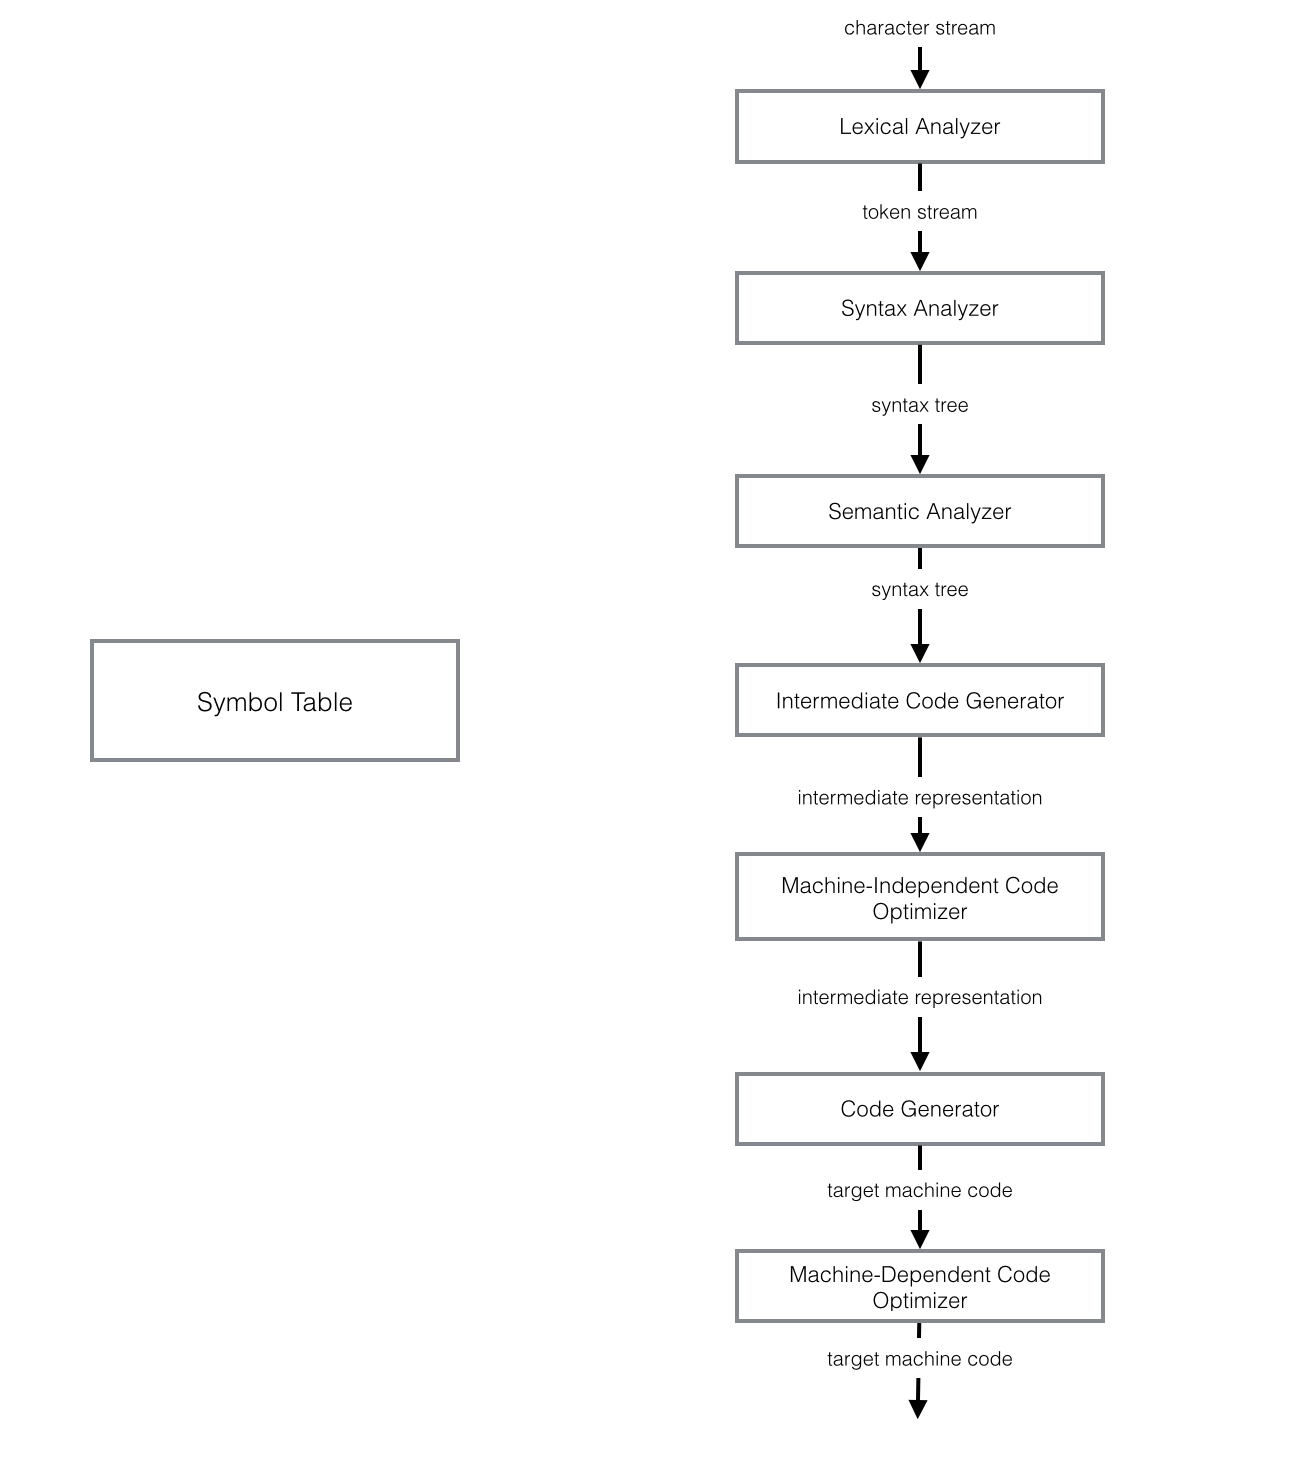
\includegraphics[width=\textwidth]{PhasesOfACompiler}
\caption{Phases of a compiler}
\label{CompilerPhases}
\end{figure}

A number if these phases are used to convert a higher level language down into a specific machine language.  In this project we already start with a machine language, which means that we do not need these phases. A program that takes an assembly language file and translates it into machine language is typically called an \textit{assembler}.

The four phases that we need for our project are Lexical Analysis, Syntax Analysis, Semantic Analysis and Code Generation. There are two of these phases, syntax analysis and semantic analysis, which are usually combined into a single phase, which is typically called a \textit{Parser}.

The first thing that we need to do is decide which programming language is the most appropriate for this component. The component takes a fixed input and always produces the same output. The component does not contain any user interaction and it does not need a user interface. These requirements led us to choose a functional language for this component. The language we chose was Haskell.

We describe how each of these phases are implemented in Haskell in the next few sections.
\section{Lexer}
The initial phase of compilation, lexical analysis, takes a stream of characters and converts them into tokens. Lexical analysis is a well know problem and there are many tools that have been created to make this task simpler. There are several lexers that already exist for Haskell and we have chosen to use a lexer called Alex\cite{alex}. 

The first thing that you need to do when creating a lexer with Alex is to determine what set of tokens you will need to create. There are several parts to the MMIX assembly language (Mmixal). The first part is the way you define what operation should be performed by the computer at a specific point in the program. This is acheived with a machine language instrustion, which is typically called an Opcode. Each instruction needs some additional parameters which informs the computer on what the instruction should operate on, these parameters are typically called operands. There are two distinct types of Opcodes in Mmixal. The first type does not vary based on what operands are used with it. The second type does vary based on the operands, and the binary representation of the Opcode is different for the different set of operands. At the end of the assembly process these instructions will be converted into a binary representation that will be stored in the memory of an MMIX computer.

The next type of instruction is used by the assembler specify either the initial state of the computer or assign internal details used as part of the assembly process. The instructions are called, in fascile 1\cite{knuth:aocp2}, pseudo instructions. These pseudo instructions do not necessarily result in anything being stored in memory.

The mmixal language also defines labels, registers, expressions and a few other things.

For this project we are using three basic groupings of tokens. The first group contains a single token, this token is for opcodes that do not vary based on their operands, we have called this token \textit{TOpCodeSimple}. The second group of tokens also contains a single token, this is the token for opcodes that do vary based on their operands, we have called this token \textit{TOpCode}. The third group contains all of the other tokens, see the code listing in Appendix~\ref{source:lexer} for a complete list of these.

When you have determined what tokens are allowed you need to describe what sequences of characters should be converted to the individual tokens. The way that you describe the tokens in Alex is to create a list of regular expressions, for each regular expression you specify which token should be created if this sequence is found.

The Alex lexer tool allows us to insert code at specific points in the process. The functions that we are using allows us to simplify the process of creating tokens.

The Alex lexer requires us to store all of these definitions in a file with an extension of \textit{x}. When all of the definitions have been completed you run the definition file through the Alex lexer tool and it generates a haskell source file that will perform the lexical analysis for you.
\section{Parser}
Once we have got a stream of tokens from the lexer, we need to perform syntax analysis and semantic analysis to make sure that the supplied program is both syntactically and semantically correct. Both of these steps are usually performed at the same time with a component called a \textit{Parser}. Parsing, like lexical analysis, is a well know problem and there are many tools that have been created to make this task simpler. These tools are generally called parser generators as they take a definition file and produce the actual parser. There are several parser generators that already exist for Haskell and we have chosen to use a parser generator called Happy\cite{happy}.

The requirement for a parser is to take a stream of tokens, make sure that the stream is syntactically and semantically correct, and then output an intermediate representation of the code that can be used to generate the final binary representation.

The first thing that we did was to design our intermediate representation, there are four different type of code lines in mmixal, as shown below.

\begin{centering}
\begin{tabular}{ l l l l }
BUF & OCTA & 0 & \textit{\%Labelled Pseudo Instruction Line}\\
 & LOC & \#100 & \textit{\%Plain Pseudo Instruction Line}\\
Main & JMP & 9F & \textit{\%Labelled Opcode Line}\\
 & STWU & n,ptop,jj & \textit{\%Plain Opcode Line}\\
\end{tabular}
\end{centering}

The way that the Happy parser generator works is that we need to create a definition file that specifies all of the syntactically and semantically correct types of statements in our language. We specify the valid statements using a context free grammar. A context free grammar contains two basic parts, an identifier and list of tokens, or identifiers, that the identifier represents. A cut down version of the parser definition file we have used can be found in Figure~\ref{cfg:happy} and a full description of the intermediate representation can be found in Appendix~\ref{iar}. 
The complete definition file can be found in Appendix~\ref{source:parser}.

\begin{figure}[ht!]
\centering
\begin{lstlisting}[basicstyle=\ttfamily\tiny]
Program         : AssignmentLines { reverse $1 }

AssignmentLines : {- empty -}        {[]}
                | AssignmentLines AssignmentLine { $2 : $1 }

AssignmentLine :: {Line}
AssingmentLine : OP_CODE OperatorList { defaultPlainOpCodeLine }
               | Identifier PI { defaultLabelledPILine }
               | Identifier OP_CODE OperatorList { defaultLabelledOpCodeLine }
               | PI { defaultPlainPILine }
               | OP_CODE_SIMPLE OperatorList { defaultPlainOpCodeLine }
               | Identifier OP_CODE_SIMPLE OperatorList { defaultLabelledOpCodeLine }
\end{lstlisting}
\caption{Sample Context Free Grammar}
\label{cfg:happy}
\end{figure}

The Happy parser generator requires us to store all of these definitions in a file with an extension of \textit{y}. When all of the definitions have been completed you run the definition file through the Happy parser generator tool and it generates a Haskell source file that will perform the syntactic and semantic analysis for you.

\section{Code Generation}
Now that we have got our program converted into an intermediate representation, in our case a list of \textit{Lines}, we need to convert this into a binary representation. The mmixal language contains a set of features called \textit{Local Labels} and processing these is the first step we perform when generating the code.
\subsection{Local Labels}
Local labels help compilers and programmers use names temporarily. They create symbols which are guaranteed to be unique over the entire scope of the input source code and which can be referred to by a simple notation. There are two parts to consider when implementing the local labels, the first is the location of the label itself, and the other is references to these labels used elsewhere in the program.

The location of a local label is specified by placing a single digit followed directly by an H, i.e. \textit{0H} as a label at the start of a line. It should be noted that an individual local label can be specified many times in a single program, when they are referenced the closest label in the required direction is used. The way that we handle this is that we rename all of the local labels to system generated labels, these labels are actually illegal for user so we know that we are not creating duplicates. The format that we use is \textit{??LS\#H*} where \# is the local label number and * is a counter. We keep note of a separate counter for each of the possible local label numbers.

The local labels are referenced as either forward or backward references, i.e. \textit{2B} specifies that we should look backwards in the code until we find a \textit{2H} local label and use that local. To achieve this we start off by creating two separate maps, one for forward references and one for backward references. Initially the forward references point to the first possible local label for the mapped digit, the backward references do not contain a reference and any use of it is a semantic error in the program. When we have these maps we iterate through the program replacing any reference to a local label with the appropriate system generated label from the specific map. We then check to see if the line actually contains a local label specification, if it does we update both the forward and backward maps with the appropriate changes. 

At the end of this process we have converted all local labels into system generated labels that can be handled as if they were ordinary user specified labels.
\subsection{Symbol Table}
As we can see in Figure~\ref{CompilerPhases} one of the data structures that we need to create as part of the code generation process is called a \textit{Symbol Table}. This is simply a map that is used to record what labels have been specified and where in the program they actually point to. To create this we simply iterate through each of the lines of the program and if they contain a label we firstly check to see if it is already present and if it does not we add the label with the current location to the symbol table.

The symbol table is used extensively in the later steps of the code generation.
\subsection{Assembler Directives}
There are a number of pseudo instructions that give the assembler instructions on how we should direct the assembly of the program. There are a number of these directive including: -
\begin{itemize}
\item \textbf{IS} Defines the value of the label to be the value of the expression.
\item \textbf{LOC} Changes the current location.
\item \textbf{GREG} Allocates a new general purpose register, see section~\ref{greg}.
\item \textbf{BYTE} Store an array of bytes in the current location. 
\item \textbf{WYDE} Store an array of wydes in the current location.
\item \textbf{TETRA} Store an array of tetrabytes in the current location.
\item \textbf{OCTA} Store an array of octabytes in the current location.
\end{itemize}
\subsection{Automatically Assigned Registers}\label{greg}
An MMix computer, by definition, contains 256 general purpose registers. The programmer can either specify which register to use directly or they can get the assembler to assign one automatically for them. A new general purpose register is allocated every time the assembler comes across a \textit{GREG} pseudo instruction. The first register that is automatically assigned is \$FE (254). Every, subsequent, automatically generated register uses the next lowest register. We have achieved this by iterating over the lines, sending along the value of the next assignable register. If the line is a GREG instruction then we change the command to one that contains the assigned register, and we then decrement the next assignable register before passing it on the the next line.
\subsection{Handling Operands}
Each opcode instructions can be supplied one, two or three operands to specify exactly what we expect to happen. The majority of opcodes can either be supplied with three registers, or it can be supplied with two registers and an immediate value. The registers could, of course, be replaced by labels which represent registers. If the line specifies three registers then the plain opcode is used when we generate the code. In the other case then when we generate the code we increment the opcode by one to let the computer know not to look for this register.

If the opcode is for a branching instruction then it will be supplied with a register and an address. For these instructions we need to determine the number of instructions between the current memory location and the memory location of the required address. We need the number of instructions, not just the difference in memory locations. This is calculated by determining the difference between the memory addresses and dividing this value by four. This address could be either ahead of, or before, the current location. If it is ahead of the current location then we use the plain opcode when generating the code. If the address is before the current location the we generate the code we increment the opcode by one.
\subsection{Generating the Output}
The final stage of the assembler is the actual outputting of the binary representation of the program. The way that we have achieved this is a two stage process. In the first stage we convert the intermediate representation of the code into a new representation of the code that makes creating the output file simpler.

\begin{lstlisting}[basicstyle=\ttfamily\small]
CodeLine {
	cl_address = 256, 
	cl_size = 4, 
	cl_code = "\240\NUL\NUL\ETB"
}
\end{lstlisting}

This representation includes the start address for this line of code, the size of the code and the binary representation of that line of code.

The final stage is to output these code lines to a file. The structure of the file contains two separate parts, the first part contains the data the needs to be placed in memory, and the second part contains the initial values that the used registers need to be set to.

To create the first part we group the code lines together into contiguous blocks. The first four bytes of this section contains the number of blocks that we have got, we then include the details for each block. The first four bytes of each block contains the start address of the block, next next four bytes of the block contains the size of the block, after this we include the actual code for the block.

The first four bytes of the second part contains the number of registers we are defining. We then include the details for each register. The first byte of the register is register number, the next eight bytes are the initial value of that register.

\section{Executable}
TODO ----- HOW WE RUN THE ASSEMBLER, WHAT THE PARAMETERS ARE \& WHAT THE OUTPUT IS
\section{Component Testing}
When it comes to testing this component we tested it these levels.
\begin{itemize}
\item We tested the lexer on its own.
\item We tested the lexer and parser together.
\item We tested the Local Label generation on its own.
\item We tested the Automatically Assigned Registers on their own.
\item We tested the Code Generation on its own.
\item We tested the component as a whole.
\end{itemize}

There are several sample programs that are written in mmixal, we used several of these when testing the assembler. The main mmixal program we used to test this component is one that determines the first 500 prime numbers. A fuller description of this program can be found at Chapter~\ref{primenumbers}.
\chapter{Virtual Machine}\label{VM}
\section{Introduction}
The majority of computers that currently exist are based on the Von Neumann Model, a description of this can be found at~\cite{vnmodel}. The main parts of a computer can be summarised as a control unit, a processing unit, memory and some for of Input/Output devices.

To execute a program a Von Neumann computer repeatedly performs the following cycle of event:
\begin{enumerate}
\item Fetch instruction from memory.\label{fec:step1}
\item Decode instruction.
\item Evaluate address.
\item Fetch operands from memory.
\item Execute operation.
\item Store results.
\item Increment the program counter.
\item Go back to step \ref{fec:step1}
\end{enumerate}

This is typically called the fetch, decode, execute cycle.

The virtual machine that we have created has most of these parts, but it relies on the GUI for all of its Input/Output devices. The virtual machine that we have created does fetch, decode, execute cycle described above.

The first thing that we need to do is decide which programming language is the most appropriate for this component. The component takes a is supplied with a program and then it is continually asked to process the next statement. There is no shared state between the VM and any other components. These requirements led us to choose a message oriented language for this component. The language we chose was Erlang.
\section{Memory}
The way that memory is organized can be considered a hierarchy, to quote Aho et al\cite{dragon}
\begin{quotation}
A memory hierarchy consists of several levels of storage with different speeds and sizes, with the levels closest to the processor being the fastest but smallest... Memory hierarchies are found in all machines. A processor usually has a small number of registers consisting of hundreds of bytes, several levels of caches containing kilobytes to megabytes, physical memory containing megabytes to gigabytes, and finally secondary storage that contains gigabytes and beyond.
\end{quotation}
For this project we will only be considering the physical memory and the registers.

Memory in an MMix computer works with patterns of 0s and 1s, commonly called \textit{binary digits} or \textit{bits}. A sequence of eight bits is commonly called a \textit{byte}. An MMix computer can also handle 16 bit sequences, called a \textit{wyde}, a 32 bit sequence, called a \textit{tetrabyte} and a 64 bit sequence, called an \textit{octabyte}.

When we are referencing memory we use \begin{math}M[k]\end{math} to denote that we are referencing the byte stored in memory address \textit{k}. When we need to reference more that one byte at a time we use the following terminology.

\textbf{Wyde}

\begin{math}
M_2[0] = M_2[1] = M[0]M[1]
\end{math}

\textbf{TetraByte}

\begin{math}
M_4[4k] = M_4[4k+1] = ... = M_4[4k+3] = M[4k]M[4k+1]...M[4k+3]
\end{math}

\textbf{OctaByte}

\begin{math}
M_8[8k] = M_8[8k+1] = ... = M_8[8k+7] = M[8k]M[8k+1]...M[8k+7]
\end{math}

Erlang contains a framework, called the open telecom platform, or OTP for short. This framework contains a number of implementations of common patterns, these patterns are called behaviours. We have simulated the memory inside the VM by using the \textit{gen\_server} OTP behaviour.

The gen\_server behaviour not only creates a new actor but it also provides functions that handle the interaction with other actors and it handles the maintenance of state within the actor.

The data structure that we are using to contain the memory is called \textit{Erlang Term Storage (ETS)}. To quote the Erlang documentation
\begin{quote}
ETS provides the ability to store very large quantities of data in an Erlang runtime system, and to have constant access time to the data.
\end{quote}

When you are using ETS you create individual tables that contain a collection of key value pair tuples. The table that we create for the memory uses the address as the key and the byte stored in the address as the value.

The data stored in an ETS table only exists while the process that owns it is in memory. When this process is terminated the table is automatically destroyed.

The other parts of the VM requests the memory server to either return or store bytes, wydes, tetrabytes or octabytes. There are a few extra requests that can be made that allow bulk operations, such as storing a completely new program.

\section{Registers}\label{registers}
An MMIX computer contains two distinct types of registers, 256 general purpose registers and 32 special purpose registers. A complete list of the special registers can be found in Figure~\ref{fig:spec_regs}. A Von Neumann computer uses a program counter to keep track of which instruction to execute next. This is not stored as a register in the definition of an MMix computer but to aid understanding of what the computer is doing we have included it as one of the special registers.

\begin{figure}[ht!]
\begin{center}
\begin{tabular}{ c l }
\head{Identifier} & \head{Description}\\
rA & Arithmetic Status Register\\
rB & Bootstrap Register\\
rC & Continuation Register\\
rD & Dividend Register\\
rE & Epsilon Register\\
rF & Failure Location Register\\
rG & Global Threshold Register\\
rH & Himult Register\\
rI & Interval Counter\\
rJ & Return-Jump Register\\
rK & Interrupt Mask Register\\
rL & Local Threshold Register\\
rM & Multiplex Mask Register\\
rN & Serial Number\\
rO & Register Stack Offset\\
rP & Prediction Register\\
rQ & Interrupt Request Register\\
rR & Remainder Register\\
rS & Register Stack Pointer\\
rT & Trap Address Register\\
rU & Usage Counter\\
rV & Virtual Translation Register\\
rW & Where Interrupted Register\\
rX & Execution Register\\
rY & Y Operand\\
rZ & Z Operand\\
rBB & Bootstrap Register\\
rTT & Dynamic Trap Address Register\\
rWW & Where Interrupted Register\\
rXX & Execution Register\\
rYY & Y Operand\\
rZZ & Z Operand\\
\end{tabular}
\end{center}
\caption{Special Registers}
\label{fig:spec_regs}
\end{figure}

We have currently only implemented a small number of these special registers.

\subsection[Arithmetic Status Register]{rA Arithmetic Status Register}\label{rA}
The Arithmetic Status Register is used to keep track of any required arithmetic events. The eight bytes in the register are used for different flags. The least significant byte contains eight event bits. These bits are commonly referred to as DVWIOUZX, the meanings of these flags can be seen in Figure~\ref{fig:ra_reg_flags}.

\begin{figure}[!ht]
\begin{center}
\begin{tabular}{ c l }
\head{Flag} & \head{Description}\\
D & Integer Divide Check\\
V & Integer Overflow\\
W & Float-to-Fix Overflow\\
I & Invalid Operation\\
O & Floating Overflow\\
U & Floating Underflow\\
Z & Division by Zero\\
X & Floating Inexact\\
\end{tabular}
\end{center}
\caption{rA Register Flags}
\label{fig:ra_reg_flags}
\end{figure}

The next least significant byte contains eight ``enable'' bits with the same name DVWIOUZX and the same meanings.  

When an exceptional condition occurs, there are two cases: If the corresponding enable bit is 0, the corresponding event bit is set to 1; but if the corresponding enable bit is 1, MMIX interrupts its current instruction stream and execute a special ``exception handler''.  Thus, the event bits record exceptions that have not been ``tripped''.

This leaves six high order bytes.  At present, only  two of those 48 bits are defined. The two bits corresponding to 
\begin{math}
2^{17}
\end{math}
and 
\begin{math}
2^{16}
\end{math}
in rA specify a rounding mode, as follows: -

\begin{center}
\begin{tabular}{ c l }
00 & Round to the nearest\\
01 & Round off\\
10 & Round up\\
11 & Round down\\
\end{tabular}
\end{center}

We have implemented the arithmetic status register as a separate actor. This actor contains three pieces of state, the rounding mode, a set of flags to keep track of the enable bits that have been set, and a set of flags to keep track of the event buts that have been set.

This actor allows us to do four this, it allows us to change the rounding mode, it allows us to potentially flag an event as having happened, it allows us to remove a flag if it exists, and it allows us to find out what the actual value is recorded in the register. The way we have implemented the get value functionality is that we have assumed that this is the last thing that happens when processing an instruction. As such we reset all of the set event flags after we have determined the current value of the register. 
\subsection{General Purpose Registers}
We are storing the general purpose registers inside a separate ETS table. This table uses the register identifier as the key and the octabyte stored in it as the value. When we start the VM, or when we send a new set of registers from the GUI, we create a new version of the ETS table.
\section{Central Processing Unit}
The Central Processing Unit (CPU) is at the heart of the virtual machine. The CPU is responsible for steps 2 - 7 in the fetch, decode, execute cycle. The first stage of fetch, decode, execute cycle that the CPU is responsible for is the decode stage. This is simple achieved with a function that pattern matches against the value and runs the relevant decoded function. 

There are many different forms of instructions that the CPU could be running, as described in Chapter~\ref{c:assembler}. 

One of the sets of instruction can be specified in one of two ways, with three registers or with two registers and an immediate value, are all implemented in a similar manner. In the case where we have three registers we obtain the value stored in the third register and then both versions functions call a shared function which performs the actual operation.

Another set of instructions are the branching instructions. These instructions all take a single register and a sixteen bit number. The instructions look at the value in the register and if it matches a boolean function then processing moves, either forward or backwards, the number of instructions specified in the sixteen bit number. The actual new location is the current location, either plus or minus, four times the specified number of instructions.

Another set of instructions are used to conditionally set the value in a register. These instructions take two registers and a number. We use the same set of boolean functions as we have in the branching instructions against the second register. If the boolean function returns true then we set the first register to the number specified, if it returns true then we leave it alone. There is another set of instructions that are identical to this however if the boolean function returns false it set the first register to zero.

The execution of MMIX programs can be interrupted in several ways. The main way that it can happen in our VM is through the TRIP and TRAP instructions. The difference between these two instructions is that TRIPs interrupt the current execution and execute some user code, whereas TRAPs interrupt the current execution and execute an operating system command. We have not implemented the TRIPs but we have implemented a small number of TRAPs.
\section{Calling the Operating System}\label{trip:trap}
There are many reasons that a program might need to interact with the operating system. It might need to read data in from secondary storage, it might need to output text to the user, it might need to be told that the current program has finished, it might need to obtain data entered in by the user.

These operations are executed through the TRAP instruction, for example

\begin{lstlisting}
TRAP 0,Fputs,StdOut
\end{lstlisting}
tells the program to look at the memory location stored in general purpose register \$255. It will assume that this memory location is the start of a null terminated string. Therefore, it will read all of subsequent memory locations until it finds a location containing 0. It will assume that all of the other values for part of the string and it will send it to the operating systems currently defined standard output.

For the purpose of our application we consider the GUI to be the operating system. The way that the VM interacts with the GUI, in the case of TRAPs, is that it creates a list of tuples, the first element of the tuple contains a symbol that is known by the GUI. The remaining elements in the tuple are the data the GUI will need to perform the operation.

There is not a definitive list of what TRAP instructions there should be, but there is a list of rudimentary I/O commands that it should execute. We have actually only implemented a couple of the possible TRAP instructions.
\section{Communication}
The way we start the VM is by executing a function that starts all of the appropriate actors and the starts a UDP server, waiting for instructions from the GUI. When the VM receive a message it processes that message and then it will send a response back to the GUI. 

The main message that we receive is the \textit{process next statement} message. This message tells the VM that we need to perform the next fetch, decode and execute cycle. The response that is sent back to the GUI from this message contains three parts. The first part is a textual representation of the decoded instruction that we have just processed. The second part is a list of tuples containing the details of any registers that have changed value. The third part is tuples containing extra messages for the GUI, these extra messages contain instructions like changes to memory locations, text to be displayed on the console.

Another message that we might receive is a request to list all of the known registers and what values they have. The response to this message is a pair tuple containing a symbol telling the GUI that we are sending it all registers and a list of pair tuples that contain the register identifier and the value of the register for all of the known registers.

All other messages that are received are processed and then we respond with a symbol telling the GUI that we have finished processing.
\section{Component Testing}
The way that we have architected the VM we were able to do some extensive unit testing.




%%%%%%%%%%%%%%%%%%%%%%%%%%%%%%%%%%%%%%%%%%%%%%%%%%%%%%%%%%%%%%%%%%%%%%%%%%%%%%%%%%%%%%%
\chapter{Graphical User Interface}
\section{Introduction}
One of the key objectives of the project chosen was to assist students understanding of how a computer program works. This objective makes the graphical user interface (GUI) a key component. A sample screenshot can be seen in Figure~\ref{screenshot}.
\begin{figure}[ht!]
\centering
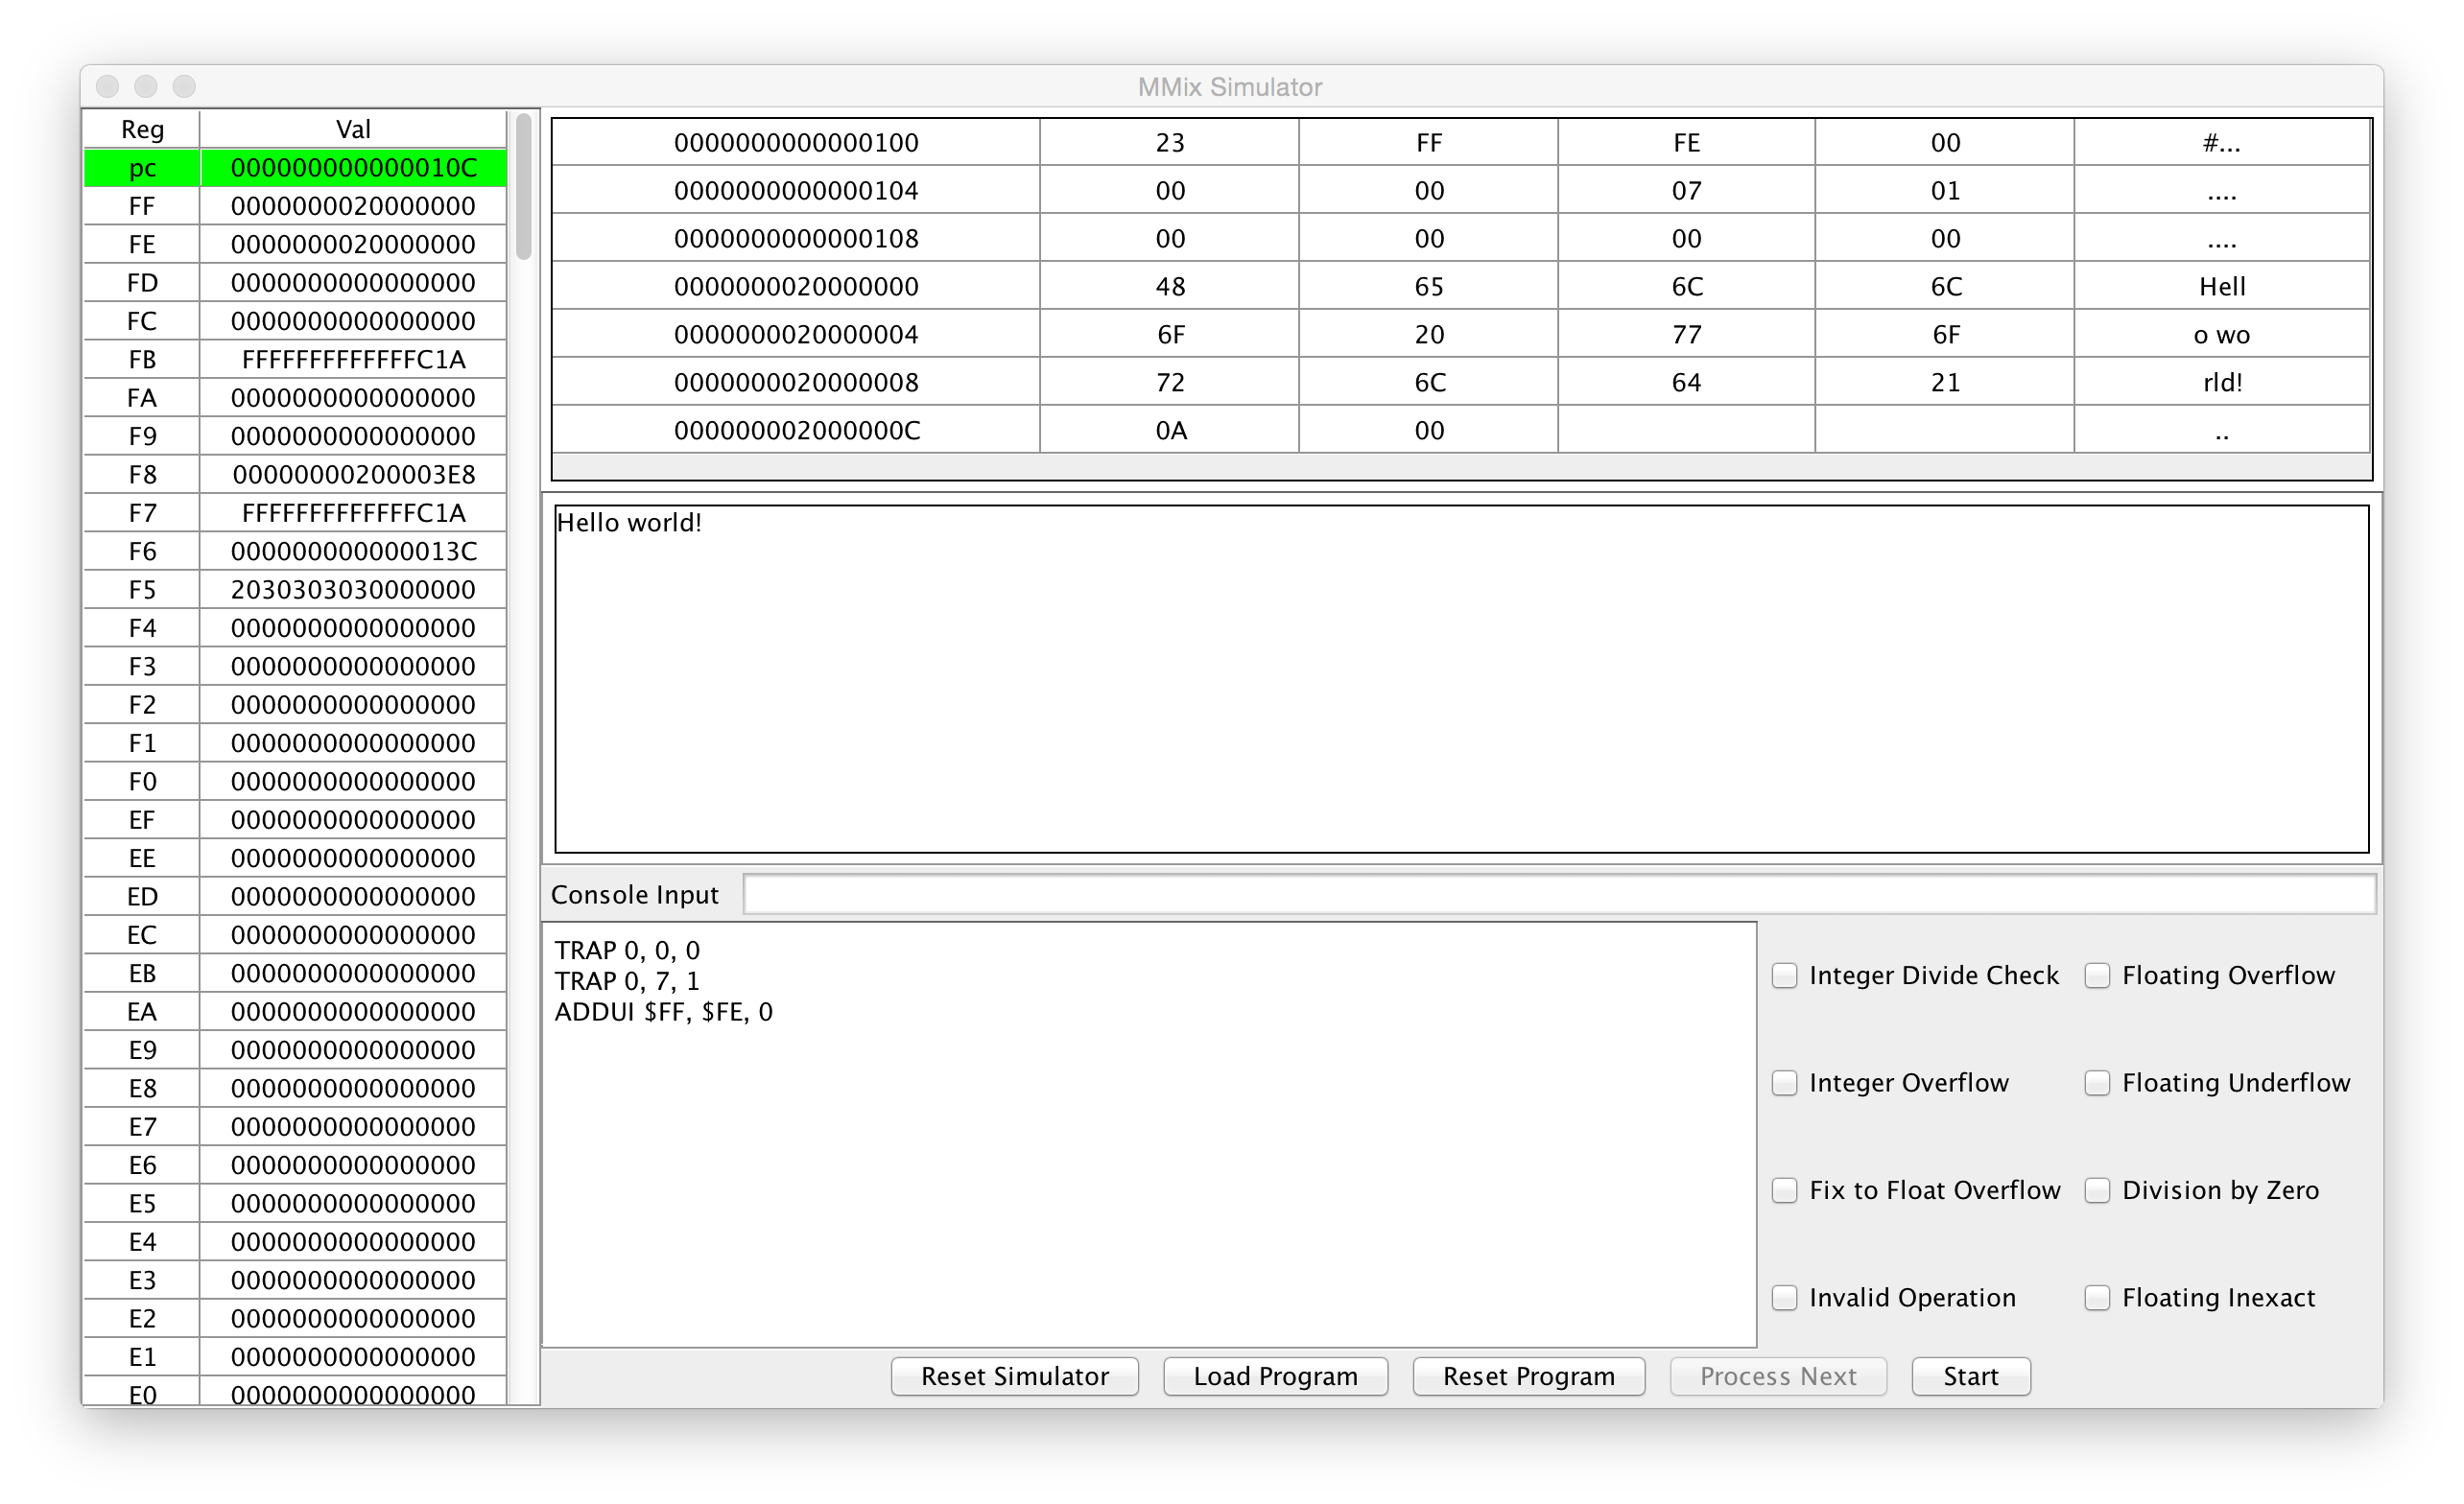
\includegraphics[width=\textwidth]{GUISample2}
\caption{GUI Sample Screenshot}
\label{screenshot}
\end{figure}

The first thing that we need to do is decide which programming language is the most appropriate for this component. This component needs to be able to display a graphical user interface and it also needs to be able to communicate with the Virtual Machine, see Chapter~\ref{VM}. These requirements led us to a more general purpose language and we chose to use Scala.
\section{User Interface Design}
We decided to split the user interface(UI) up into a number of smaller regions, which are typically called panels. 
\subsection{Console Panel}
The console panel is a fairly simple panel that simulates the interaction between the computer and the end user. This panel contains two separate areas, the main area shows details that the programmer wants to inform the user about. The other area allows the user to enter some data and send it to the program, when they are so prompted.
\subsection{Controls Panel}
The controls panel is the area of the GUI that contains the buttons which allow the user to interact with the simulator. The controls panel contains the following buttons: -
\begin{itemize}
\item \textbf{Reset Simulator} -- This button completely resets the simulator, removing any currently loaded program from memory.
\item \textbf{Load Program} -- This button allows the user to choose a file that contains the binary representation of an MMIX program. This program will then be loaded in from the file and passed on to the virtual machine. When this process has finished the application will be ready to start simulating the program. This process obviously has to be able to understand the binary representation of the mmixal program that our assembler creates.
\item \textbf{Reset Program} -- This button will reset the GUI and the virtual machine back to the same state it was in when the application was first loaded.
\item \textbf{Process Next} -- This button, when enabled, will process the next available statement.
\item \textbf{Start / Stop} -- This button allows the GUI to automate the processing of the next statements, freeing the user up from having to constantly press the process next button.
\end{itemize}
\subsection{Main State Panel}
The main state panel contains two separate areas, the main area contains a list of all of the instructions that the VM has processed. This list is displayed in reverse order so that the last statement executed is at the top of the list. The other area shows a number of flags, these flags are stored in the arithmetic status register, which is described in section~\ref{rA}.
\subsection{Memory Panel}
The memory panel contains a table that describes the current state of the memory in the VM. The each row in the table starts with a column the tells the user the starting memory address for this row. The next four columns give a hexadecimal representation of the contents of those memory locations. The final column contains an ASCII representation of the data in those four memory locations, if the cell contains a non printable ASCII character then it is substituted with a `.'. 

If the processing of an instruction changes the content of a memory location then those memory locations are highlighted in green.
\subsection{Registers Panel}
The registers panel contains the current values stored in all of the general purpose and special registers. It also includes the current value of the additional program counter register we are using to keep count of the location of the next instruction to be processed.

If the processing of an instruction changes the content of a register then those registers are highlighted in green.
\section{Asynchronous UI Programming with Actors}
The development of a graphical user interface will always contain a few non-functional requirements, one that should always be present is that the GUI should be responsive. We mean, by this, that the GUI should always respond to what the user does with it, no matter what processing it is also doing at the same time. This has traditional been the domain of multi-threaded programming, however there is now a new approach available to us, we can use an actor library. 

When we use an actor library you gain a mechanism for easily handling concurrency and parallelism.  A highly regarded actor library that is available in Scala is called Akka~\cite{akka}. To quote the Akka website: -

\begin{quotation}
Actors give you:

\begin{itemize}
\item Simple and high-level abstractions for concurrency and parallelism.
\item Asynchronous, non-blocking and highly performant event-driven programming model.
\item Very lightweight event-driven processes (several million actors per GB of heap memory).
\end{itemize}
\end{quotation}

The way that we have designed the GUI is that we have created a separate actor for each of the panels and a separate actor that is responsible for communicating with the virtual machine. The panel actors are responsible for both updating the panels with information from the VM and handling any input from the users. The virtual machine actor is responsible for communicating with the VM.
\section{Communication}
There are two types of communication that we need to handle in the project, communication between the GUI and the BM, along with communication between the various UI panels.
\subsection{GUI to VM Communication}
We need a mechanism for transferring data and commands between the GUI written in Scala and the VM written in Erlang. There is a built in function inside Erlang which will convert a term, which is the name Erlang uses for a data structure, into binary. This function is called \textit{term\_to\_binary} and it takes a value as a parameter. The function creates a binary representation based on a fixed format the can be found on the Erlang website~\cite{term_to_binary}.

We have written an object, in Scala, that will perform the same translation. It will convert binary streams from Erlang into Scala data structures and it will convert Scala data structures into a binary stream that Erlang can understand. This object has been embedded inside the Virtual Machine Actor, the full source code is available in Appendix~\ref{source:vm_actor}.

This object allows us the ability to marshal data structures between the two components but we also need to handle the actual transferral action. We have decided to, initially, require that both the GUI and VM processes should run on the same physical machine. This requirement allows us to simple create a UDP connection between the two processes.
\subsection{UI Panel Communication}
The communication between the UI panels, and the virtual machine actor all happens with Akka messages. As an example when we ask the VM to process the next statement it will respond with not only all of the things that have changed but what instruction was executed and all some updates to the console. This results in the virtual machine actor sending messages to the main state panel actor, the memory panel actor, the registers panel actor and potentially the console panel actor.
\section{Component Testing}



\chapter{Simulator Application}
\section{Introduction}
In the previous chapters we have described the individual components that make up the Simulator Application.
\section{Integration Testing}
\begin{centering}
\begin{tabular}{ l l l }
 & LOC & Data\_Segment\\
 & GREG & @\\
txt & BYTE & ``Hello world!'',10,0\\
\\
 & LOC & \#100\\
\\
Main & LDA & \$255,txt\\
 & TRAP & 0,Fputs,StdOut\\
 & TRAP & 0,Halt,0\\
\end{tabular}
\end{centering}
\subsection{Generate Prime Numbers Sample Application}
\label{primenumbers}
\chapter*{Conclusion}
\addcontentsline{toc}{chapter}{Conclusion}
We found that having a single developer 

Pattern Matching

Lists

Tuples

\section*{Possible Future Enhancements}
\addcontentsline{toc}{section}{Possible Future Enhancements}
Extra TRAP instructions.

Extra special registers.

Directly link the GUI with the Assembler.

\nocite{*}
\bibliographystyle{alpha}
\bibliography{bibtex}
\addcontentsline{toc}{chapter}{References}
\begin{appendices}
\noappendicestocpagenum
\addappheadtotoc 
\chapter{Source Code}
\section{Assembler}\label{source:assembler}
\subsection{Lexer}\label{source:lexer}
\lstinputlisting[language=Haskell,basicstyle=\ttfamily\tiny]{assembler/MMix_Lexer.x}
\subsection{Parser}\label{source:parser}
\lstinputlisting[language=Haskell,basicstyle=\ttfamily\tiny]{assembler/MMix_Parser.y}
\subsection{Symbol Table}\label{source:SymbolTable}
\lstinputlisting[language=Haskell,basicstyle=\ttfamily\tiny]{assembler/SymbolTable.hs}
\subsection{Common Data Types}\label{source:DataTypes}
\lstinputlisting[language=Haskell,basicstyle=\ttfamily\tiny]{assembler/DataTypes.hs}
\subsection{Expressions}\label{source:Expressions}
\lstinputlisting[language=Haskell,basicstyle=\ttfamily\tiny]{assembler/Expressions.hs}
\subsection{Locations}\label{source:locations}
\lstinputlisting[language=Haskell,basicstyle=\ttfamily\tiny]{assembler/Locations.hs}
\subsection{Registers}\label{source:registers}
\lstinputlisting[language=Haskell,basicstyle=\ttfamily\tiny]{assembler/Registers.hs}
\subsection{Code Generation}\label{source:codegen}
\lstinputlisting[language=Haskell,basicstyle=\ttfamily\tiny]{assembler/CodeGen.hs}
\subsection{External Interface}\label{source:main}
\lstinputlisting[language=Haskell,basicstyle=\ttfamily\tiny]{assembler/Main.hs}
\section{Graphical User Interface}
\subsection{Scala Build Tool}\label{source:sbt}
\lstinputlisting[basicstyle=\ttfamily\tiny]{gui/build.sbt}
\subsection{Console Panel}\label{source:console_panel}
\lstinputlisting[basicstyle=\ttfamily\tiny]{gui/ConsolePanel.scala}
\subsection{Controls Panel}\label{source:controls_panel}
\lstinputlisting[basicstyle=\ttfamily\tiny]{gui/ControlsPanel.scala}
\subsection{Main Form}\label{source:main_form}
\lstinputlisting[basicstyle=\ttfamily\tiny]{gui/main_form.scala}
\subsection{Main State Panel}\label{source:main_state_panel}
\lstinputlisting[basicstyle=\ttfamily\tiny]{gui/MainStatePanel.scala}
\subsection{Memory Panel}\label{source:memory_panel}
\lstinputlisting[basicstyle=\ttfamily\tiny]{gui/MemoryPanel.scala}
\subsection{MMix File}\label{source:mmix_file}
\lstinputlisting[basicstyle=\ttfamily\tiny]{gui/MMixFile.scala}
\subsection{Register Panel}\label{source:register_panel}
\lstinputlisting[basicstyle=\ttfamily\tiny]{gui/RegisterPanel.scala}
\subsection{Utilities}\label{source:utilities}
\lstinputlisting[basicstyle=\ttfamily\tiny]{gui/Utilities.scala}
\subsection{Virtual Machine Actor}\label{source:vm_actor}
\lstinputlisting[basicstyle=\ttfamily\tiny]{gui/VirtualMachineActor.scala}
\section{Virtual Machine}
\subsection{Branch}\label{source:vm_branch}
\lstinputlisting[language=erlang,basicstyle=\ttfamily\tiny]{vm/branch.erl}
\subsection{Communication}\label{source:vm_comm}
\lstinputlisting[language=erlang,basicstyle=\ttfamily\tiny]{vm/comm.erl}
\subsection{CPU Main Header}\label{source:vm_cpu_header}
\lstinputlisting[language=erlang,basicstyle=\ttfamily\tiny]{vm/cpu.hrl}
\subsection{CPU Execute Statment}\label{source:vm_cpu_execute}
\lstinputlisting[language=erlang,basicstyle=\ttfamily\tiny]{vm/cpu_execute.hrl}
\subsection{CPU}\label{source:vm_cpu}
\lstinputlisting[language=erlang,basicstyle=\ttfamily\tiny]{vm/cpu.erl}
\subsection{Memory}\label{source:vm_memory}
\lstinputlisting[language=erlang,basicstyle=\ttfamily\tiny]{vm/memory.erl}
\subsection{rA Register}\label{source:vm_register_ra}
\lstinputlisting[language=erlang,basicstyle=\ttfamily\tiny]{vm/register_ra.erl}
\subsection{Registers}\label{source:vm_register}
\lstinputlisting[language=erlang,basicstyle=\ttfamily\tiny]{vm/registers.erl}
\subsection{Trap}\label{source:vm_trap}
\lstinputlisting[language=erlang,basicstyle=\ttfamily\tiny]{vm/trap.erl}
\subsection{Utilities}\label{source:vm_utilities}
\lstinputlisting[language=erlang,basicstyle=\ttfamily\tiny]{vm/utilities.erl}

\chapter{Intermediate Assembler Representations}\label{iar}
\section{Definitions}
\section{Test Application}
\subsection{Sample Test MMIXAL Code}
The sample mmixal application I am using to test the system is taken from Fascile 1\cite{knuth:aocp2}.  The complete code listing is: -

\begin{CenteredBox}
\lstinputlisting[basicstyle=\ttfamily\tiny]{primes.mms}
\end{CenteredBox}
\subsection{Parsed Sample File}
The final intermediate representation of the parsed source code for the test application is: -

\lstinputlisting[language=Haskell,basicstyle=\ttfamily\tiny]{parsed_example.hs}
\end{appendices}
\clearpage
\addcontentsline{toc}{chapter}{Index}
\printindex
\end{document}

